\begin{problem}{5}
    How do circles centered on the origin in the z-plane transform for
    \begin{enumerate}
        \item $$w_1(z) = z + \frac{1}{z}$$ 
        \item $$w_2(z) = z - \frac{1}{z}$$ 
    \end{enumerate}
    What happens when $|z| \rightarrow 1$?
\end{problem}
\subsection*{Solución}
Expresando $z = x + iy$, donde $x = r\cos\theta$ y $y = r\sin\theta$.
\begin{enumerate}
    \item  
    \begin{gather*}
        w_1(z) = x + iy + \frac{1}{x+iy} = x + iy + \frac{x-iy}{x^2+y^2}
    \end{gather*}
    separando en su parte real, e imaginaria 
    \begin{gather*}
        w_1(z) = x\left(1 + \frac{1}{x^2+y^2}\right) + iy\left(1 - \frac{1}{x^2+y^2}\right)
    \end{gather*}
    remplazando los respectivos valores de $x$ y $y$

    \begin{gather}
        w_1(z) = r\cos\theta\left(1 + \frac{1}{r}\right) + ir\sin\theta\left(1 - \frac{1}{r}\right)
    \end{gather}
    ahora la función $w_1(z)$ debe tener la forma funcional $w_1(z) = u(r,\theta) + iv(r,\theta)$, igualando las partes linealmente independientes.
    \begin{gather*}
        u(r,\theta) = r\cos\theta\left(1 + \frac{1}{r}\right) \quad\quad v(r,\theta) = r\sin\theta\left(1 - \frac{1}{r}\right)
    \end{gather*}
    elevando cada término al cuadrado
    \begin{gather*}
        u^2 = r^2\cos^2\theta\left(1 + \frac{1}{r}\right)^2 \quad\quad v(r,\theta) = r^2\sin^2\theta\left(1 - \frac{1}{r}\right)^2
    \end{gather*}
    y recordando que $\cos^2\theta + \sin^2\theta = 1$, se obtiene 
    
    \begin{result}
        \begin{gather}
            \frac{u^2}{r^2\left(1 + \frac{1}{r}\right)^2} + \frac{v^2}{r^2\left(1 - \frac{1}{r}\right)^2}  = 1 \quad (r\neq 1)
        \end{gather}
    \end{result}
    resulta se la ecuación de una elipse donde el semieje mayor está sobre $u$, realizando la gráfica.

    \begin{figure}[h]
        \centering
        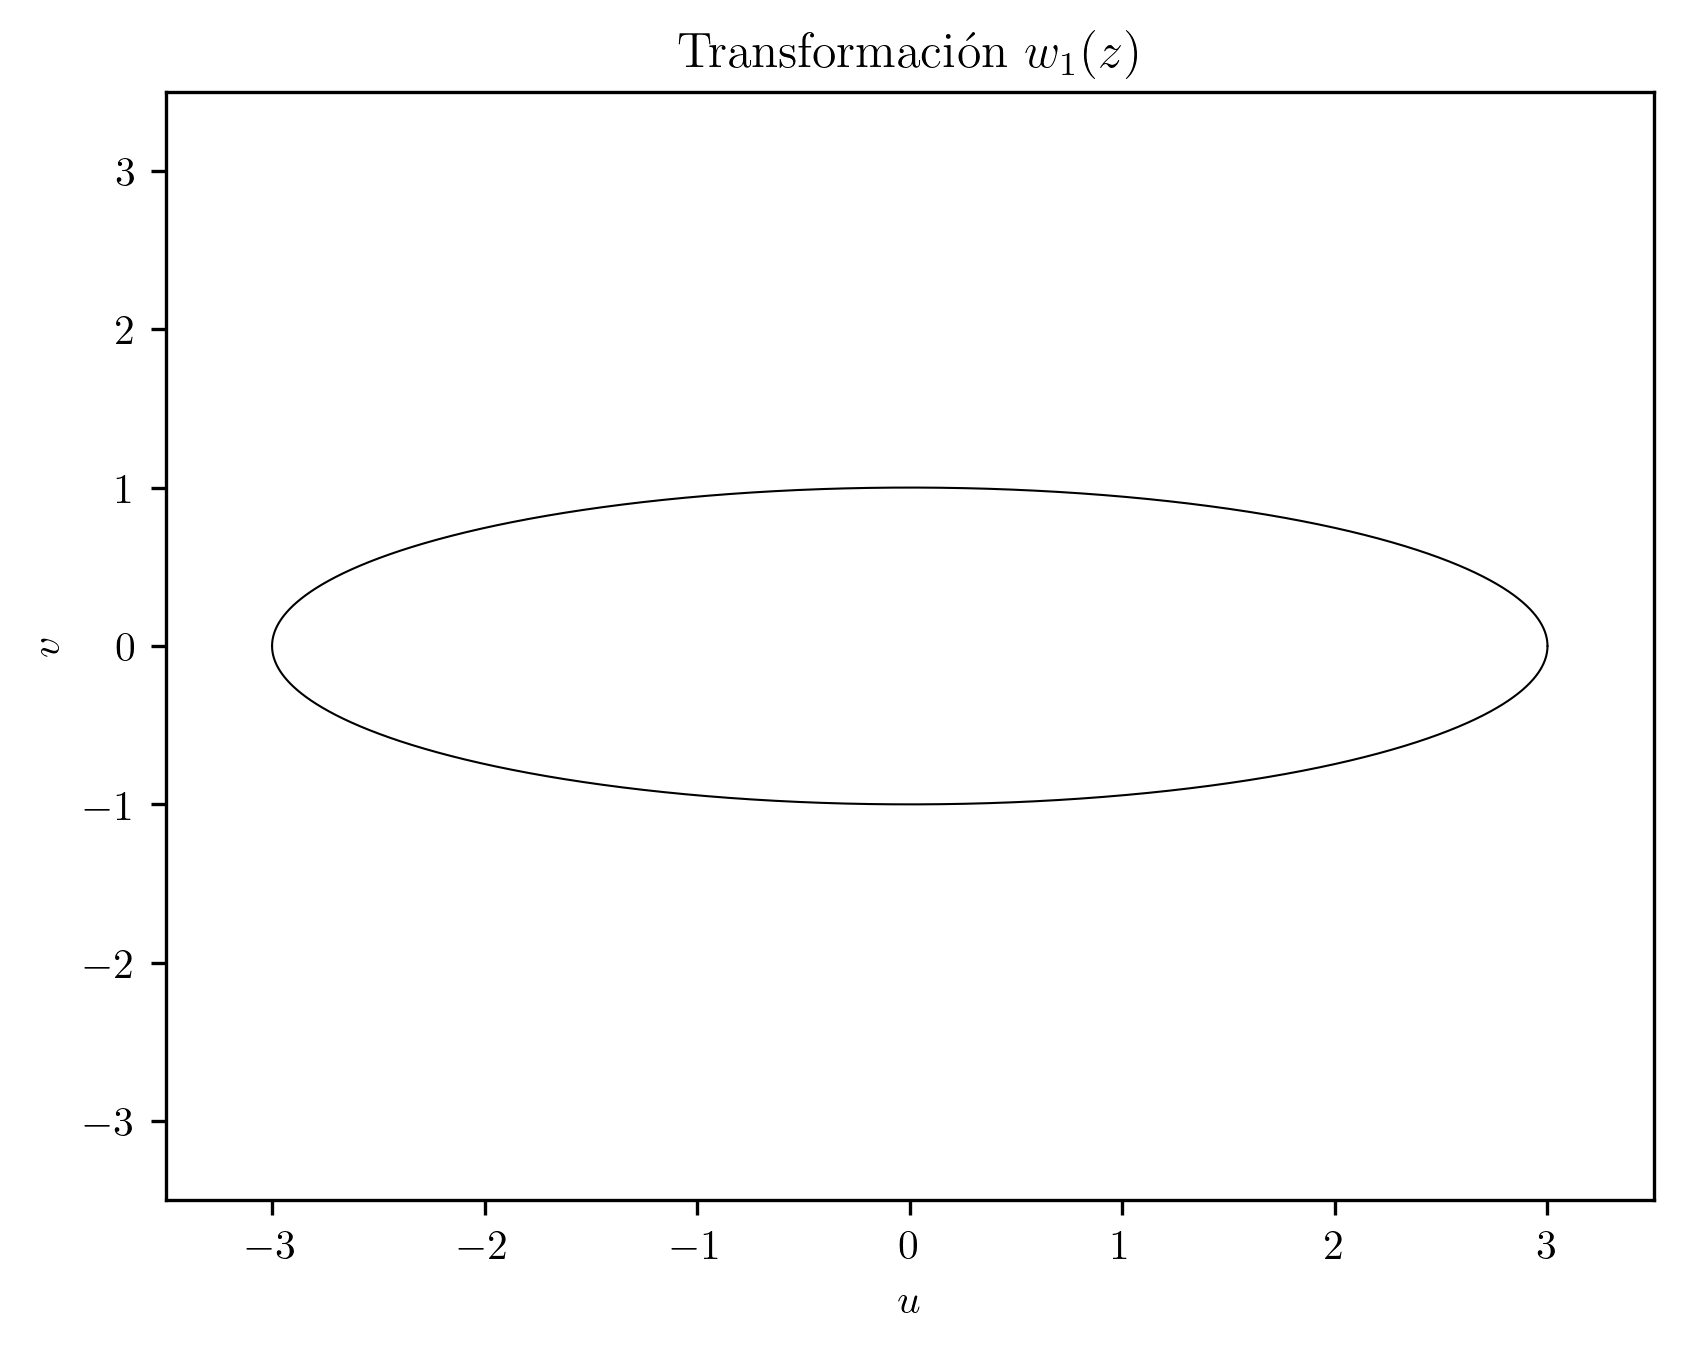
\includegraphics{imgs/w1.png}        
    \end{figure}

    \item 
    \begin{gather*}
        w_2(z) = x + iy - \frac{1}{x+iy} = x + iy - \frac{x-iy}{x^2+y^2}\\
        w_2(z) = x\left(1 - \frac{1}{x^2+y^2}\right) + iy\left(1 + \frac{1}{x^2+y^2}\right)
    \end{gather*}
    remplazando los respectivos valores de $x$ y $y$

    \begin{gather}
        w_1(z) = r\cos\theta\left(1 - \frac{1}{r}\right) + ir\sin\theta\left(1 + \frac{1}{r}\right)
    \end{gather}
    igualando a la parte real e imaginaria de la forma funcional de $w_2(z)$ 
    \begin{gather*}
        u(r,\theta) = r\cos\theta\left(1 - \frac{1}{r}\right) \quad\quad v(r,\theta) = r\sin\theta\left(1 + \frac{1}{r}\right)
    \end{gather*}
    parametrizando una función en términos de la otra se obtiene la trayectoria que traza $w_2(z)$ en el plano complejo.
    \begin{result}
        \begin{gather}
            \frac{u^2}{r^2\left(1 - \frac{1}{r}\right)^2} + \frac{v^2}{r^2\left(1 + \frac{1}{r}\right)^2}  = 1 \quad (r\neq 1)
        \end{gather}
    \end{result}
    esta es la ecuación de una elipse, donde el semieje mayor esta en dirección de $v$

    \begin{figure}[h]
        \centering
        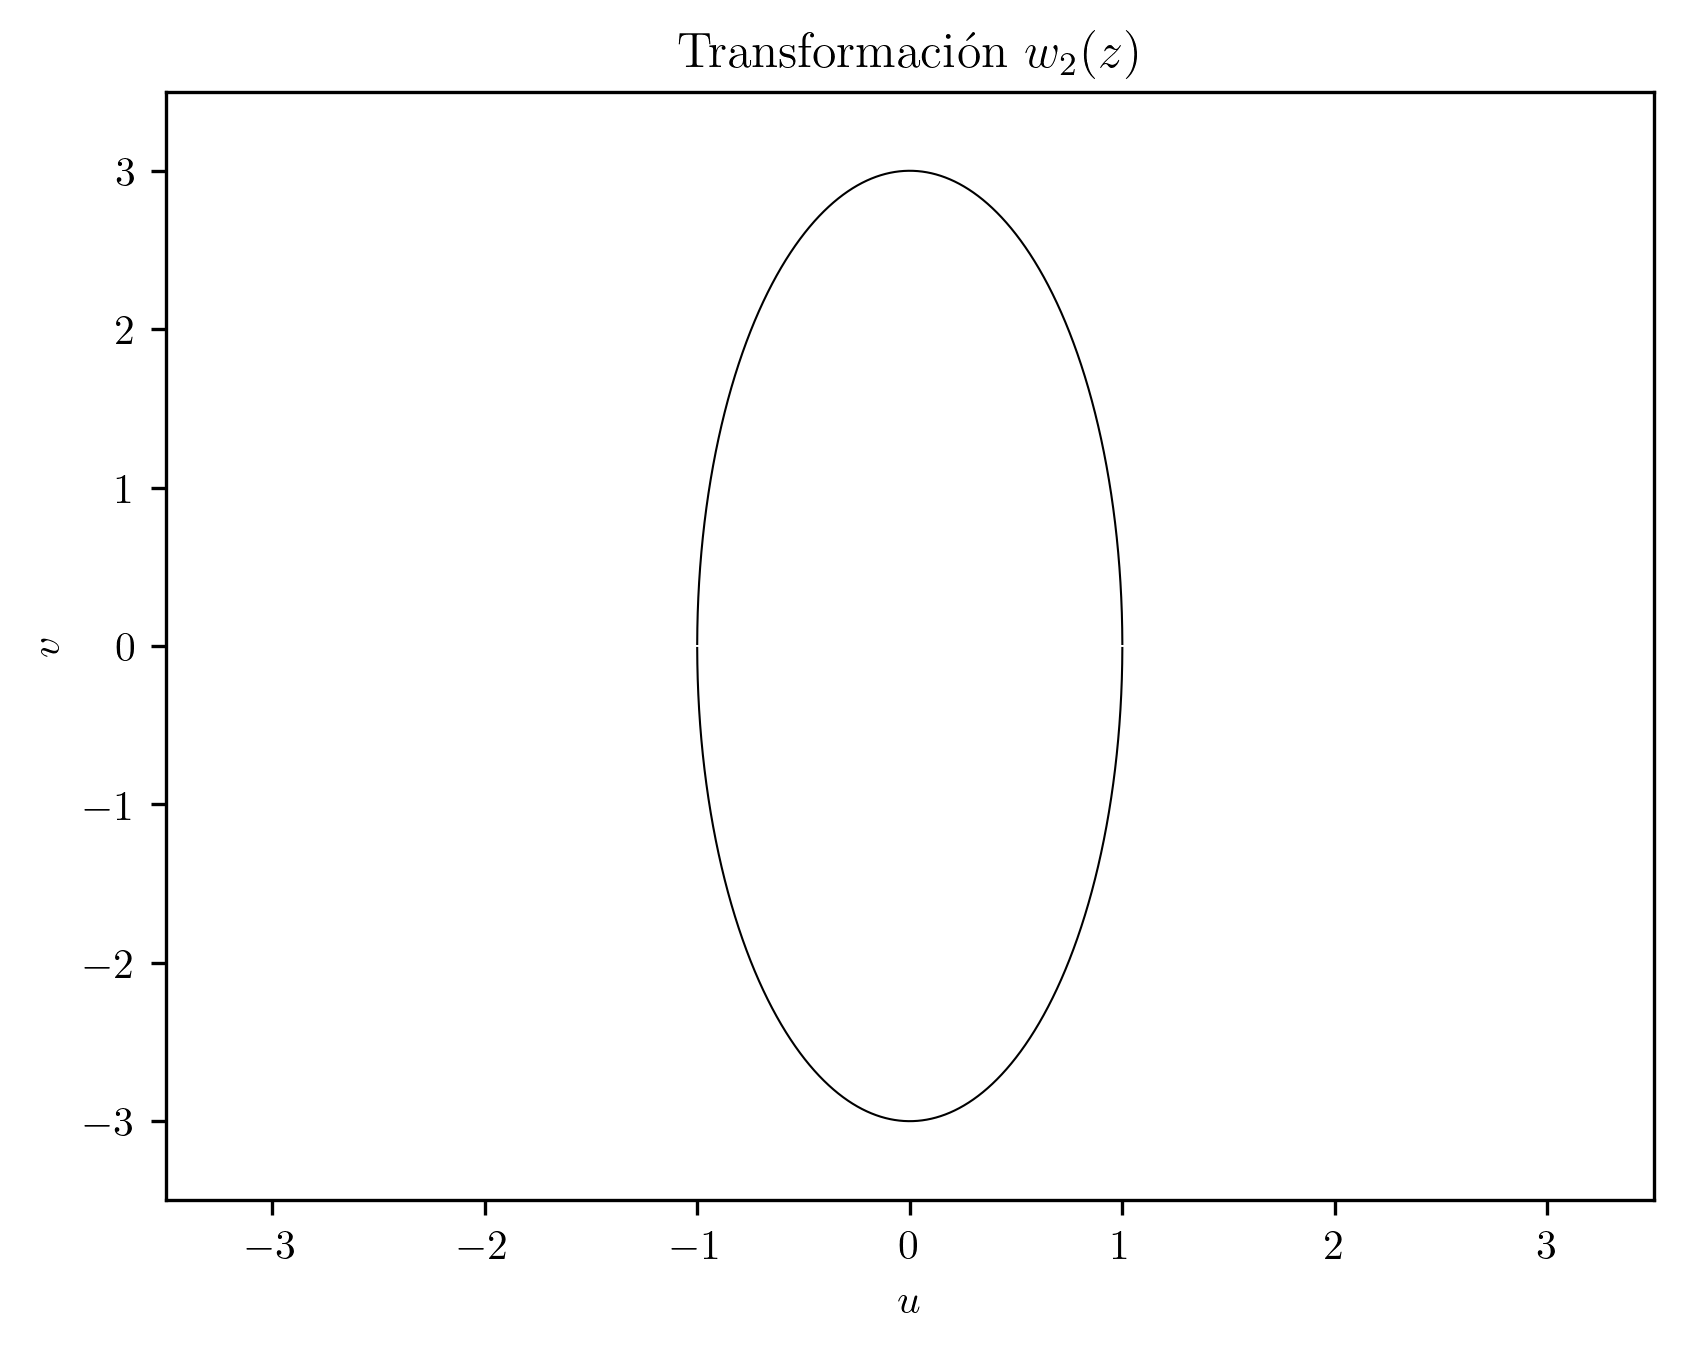
\includegraphics{imgs/w2.png}        
    \end{figure}
\end{enumerate}